\documentclass[12pt,letterpaper]{article}
\usepackage[utf8]{inputenc}
\setlength{\parindent}{0 pt}
\usepackage{amsmath}
\usepackage{amsfonts}
\usepackage{amssymb}
\usepackage{graphicx}
\usepackage{multicol}
\usepackage{changepage}
\usepackage{float}
\usepackage{cite}
\usepackage{url}

\usepackage[left=2.50cm, right=2.50cm]{geometry}
\author{Rafael Hernández Sánchez}
\title{OptoAcopladores y Relevadores}

\begin{document}
	\pagestyle{plain}{
	\pagestyle{empty}
	
	\begin{center}
		\par\vspace{3cm}
		{
			\Huge\textbf{\textit{Universidad politécnica de la zona metropolitana de Guadalajara}}
		}
		\par\vspace{0.35cm}
		{
			\Large{\textbf{CARRERA:} Ingenieria en Mecatrónica \\ \textbf{MATERIA:} Sistemas Electrónicos de Interfaz \\ \textbf{MAESTRO:} Carlos Enrique Morán Garabito \\ \textbf{GRADO Y GRUPO:} 4-B}
		}
		\par\vspace{1cm}
		{
			\large\textbf{Práctica 2: Opto Acopladores y Reveladores}
		}
		\par\vspace{1cm}
		{
			\large\textbf{Rafael Hernández Sánchez \\ 04/10/19 \\}
		}
		
\includegraphics[scale=0.7]{UPZMG_Mecatr_nica}
		
		\par\vspace{3cm}
		

	\end{center}
	\clearpage
		\newpage
}
\section{OBJETIVO}
	Abordar la teoría de optoacopladores y relevadores mediante una práctica con el fin de comprobar y comprender su funcionamiento.

	\section{\textbf{LISTA DE MATERIALES}}
	\begin{itemize}
	\item Protoboard
	\item Resistencias
	\item Reveladores
	\item Leds
	\item Cables de Proto
	\item Fuente 
	\item Octo. 4n25
	\item n2222
	\item Diodos 007
	\item Arduino Uno
	\item Buttons
	\end{itemize}
	
\section{\textbf{MARCO TEÓRICO}}
	Un optoacoplador es un componente electrónico que se utiliza como transmisor y receptor óptico (de luz), es decir pueden transmitir de un punto a otro una señal eléctrica sin necesidad de conexión física ni cables, mediante una señal luminosa. Por eso también se llaman OptoInterruptor.\\
	La figura que se muestra enseguida, es un optoacoplador 4N35 formado por un led y un fototransistor. La tensión de la fuente de la izquierda y la resistencia en serie establecen una corriente en el led emisor cuando se cierra el interruptor S1. Si dicha corriente proporciona un nivel de luz adecuado, al incidir sobre el fototransistor lo saturará, generando una corriente en R2. De este modo la tensión de salida será igual a cero con S1 cerrado y a V2 con S1 abierto.\\

	\begin{center}
		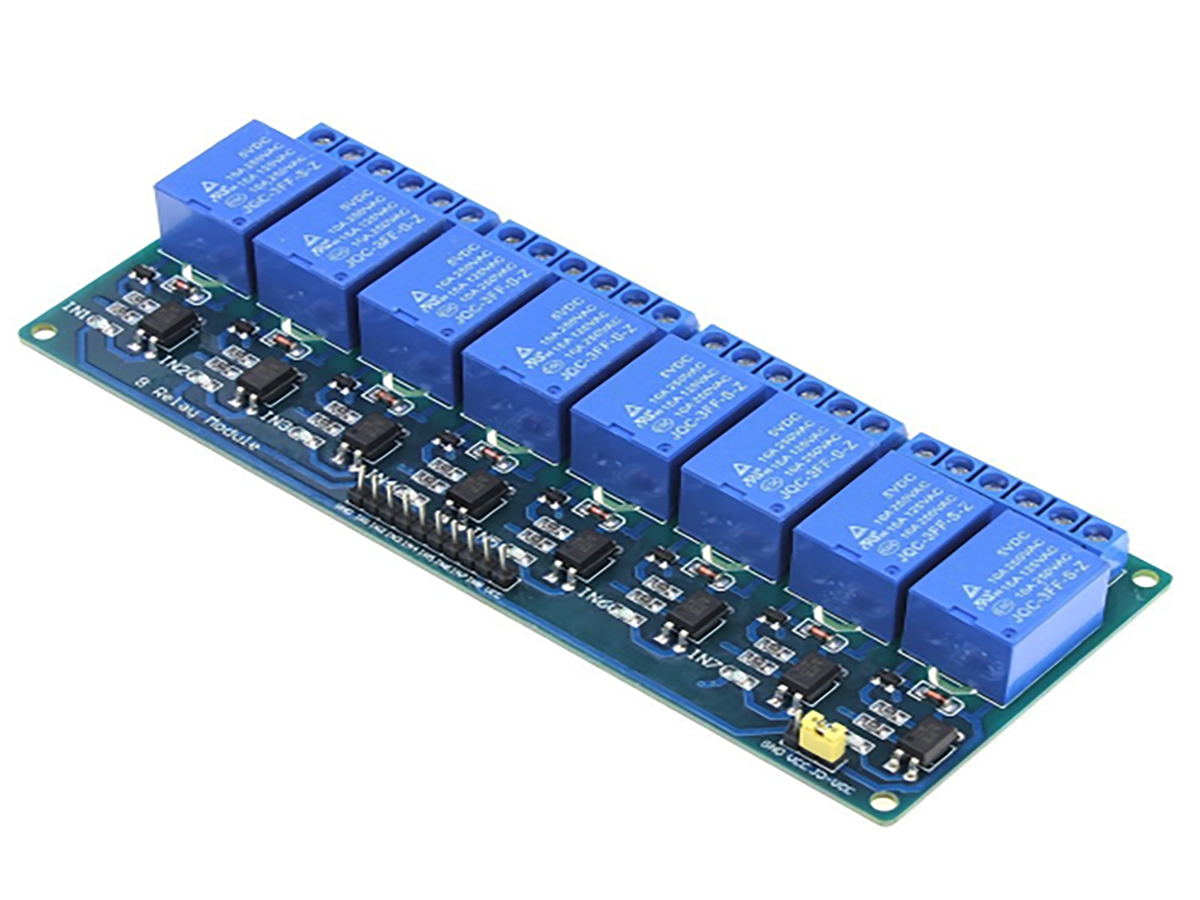
\includegraphics[scale=0.2]{Modulo-rele-8-canales-con-optoacoplador-arduino-colombia-precio}
	\end{center}


	Es decir si la tensión de entrada varía, la cantidad de luz también lo hará, lo que significa que la tensión de salida cambia de acuerdo con la tensión de entrada. De este modo el dispositivo puede acoplar una señal de entrada con el circuito de salida, aunque hay que tener en cuenta que las curvas tensión/luz del led no son lineales, por lo que la señal puede distorsionarse. \\
	La ventaja fundamental de un optoacoplador es el aislamiento eléctrico entre los circuitos de entrada y salida. \\
\section{PRINCIPALES USOS}
Además de para aislar circuitos, se pueden utilizar optoacopladores para: 
	\begin{itemize}
		\item Interfaces en circuitos lógicos.
		\item Interfaces entre señales de corriente alterna y circuitos lógicos.
		\item En sistemas de recepción (telefonía).
		\item Control de potencia.
		\item A modo de relé.
	\end{itemize}
\newpage
\section{PRACTICA}
	El modo más sencillo para activar un relé con un circuito electrónico de control es a través
	de un transistor NPN conectado como se ve en la figura. El transistor, conectado de este
	modo, cierra el circuito poniendo a masa el terminal de la bobina mientras que el otro terminal
	se encuentra conectado a positivo.\\
	El sistema que analizaremos funciona correctamente con todas las tecnologías citadas.\\\\
	\begin{center}
	(imagen1)
	\end{center}
	Estado del circuito con tensión de control a 0 volt.\\\\
	El ejemplo ilustrado funciona de este modo: cuando la salida del circuito de control es baja
	(0V) lo será también la base del transistor (indicada en la figura con la letra b) y por lo tanto
	este no dejará pasar corriente entre emisor y colector (indicados en la figura como e y c) para activar la bobina del relé (en la figura, la parte de los contactos del relé la he hecho con color
	gris porque no es importante para la descripción del funcionamiento. 

\subsection{LA RESISTENCIA A MASA}
	Aunque si no es imprescindible, es una buena costumbre agregar una resistencia entre la base
	del transistor y masa como se ve en la figura. Sirve fundamentalmente para evitar que el transistor pueda activar en modo errático el relé si nuestra entrada de control se encuentra en
	un estado indefinido. Esta situación se puede crear cuando un microcontrolador está en fase
	de inicialización y sus salidas no se encuentran todavía mapeadas (y por lo tanto en alta
	impedancia).
	\begin{center}
		(imagen2)
	\end{center}
	En este trabajo de configuración, el programa debe indicar
	cuales son las patitas (pins) que serán usadas como entradas y cuales como salidas. Hasta que
	no termina, estos pins se encuentran "desconectados" y por lo tanto la base de nuestro
	transistor también lo será. Esto puede provocar activaciones erráticas del relé.
\section{REPORTE}
	\subsection{PARTE 1}
	Una vez analizado el tema, ahora solo quedaba por hacer el circuito deseado en la practica para lograr realizar lo objetivos. como se vera en esta practica como primer paso fue construir la primera parte del circuito por el cual en estos se tiene que enviar las señales de entrada para el arduino. el cual quedo de la siguiente manera solamente de usar unas resistencias utilisamos leds para saber cual entrada estaba encendida.
	\begin{center}
		(imagen3)
	\end{center}
	\subsection{PARTE 2}
	Como segunda para se tuvo que realizar las salidas con los relevadores con el cual el objetivo era al realizar que cuando reciba la señal uno encendiera el led de la salida uno. asi has lograr con los tres. con el cual este quedo de la siguiente manera con el cual en este se de utilidad a los relevadores y n2222 al igual que los diodos.\\
	\begin{center}
		(imagen4)
	\end{center}
	\subsection{PARTE 3}
	Como ultima parte fue realizar el programa para arduino el cual este cuando reciba la señal 1 de una salida de 1 para encender con coincidencia los relevadores y así encender el led deseado. Por  el cual el objetivo de esta es la utilización de los n2222 que den el paso al recibir la señal.\\
	Como se muestra enseguida es el programa de arduino que se utilizo.
	\begin{center}
		(imagen5)
	\end{center}

\section{CALCULOS PARA LAS RESISTENCIAS}

	\begin{center}\textbf
		{
			$ R1=12v/0.060A=200ohm $\\
			$ R2=12v/0.050A=100ohm $\\
			$ R3=12v/0.030A=400ohm $\\
			$ R4=(12v-1.9)/0.030A=10.1/0.030A=336.6ohm $\\
		}
		
	\end{center}
	
\section{RESULTADOS}
	Como resultados fueron correctos, en el cual objetivo deseado fue cumplido asi como tambien se logro comprender el tema.\\
	Enseguida se mostraran los resultos con las señales de entradas y salidas correctas.\\\\
	
	(imagenef1),(imagenf2)(imagenf3)
	
\section{CONCLUCIÒN}
	En conclusión se que si llegar a preocupar las perturbaciones eléctricas que pueden ocasionar una carga a tu sistema, es mejor lo recomendable el uso de fuentes de alimentación separadas y usar un optoacoplador para evitar problemas al igual facilitar el uso del propósito. Recordando que este dispositivo no puede controlar mucha potencia. Entonces es necesario usarlo con un elemento que pueda controlar mayor potencia asi como el usar el octo adecuado. El optoacoplador es una de las mejores opciones para aislar dos etapas eléctricas para circuitos.\\
	Asi como tambien logramos comprender todos los tipos de problemas que tuvimos como los problemas con el programa y el mal manejo del voltaje puede llegar a quemar los n2222.
	
\end{document}	

\section{BIBLIOGRAFIAS}

	\cite{https://library.e.abb.com/public/c21957d57c50afeec125718c005edc59/Reles
	\cite{https://www.areatecnologia.com/electronica/optoacoplador.html}
	\cite{https://hetpro-store.com/TUTORIALES/optoacoplador/}




